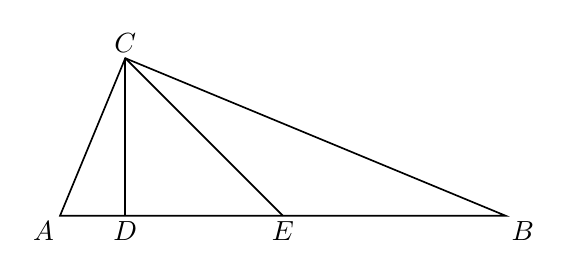
\begin{tikzpicture}[x=1cm,y=1cm,font=\normalsize,
 geometry edge/.style={solid,line width=.6pt},
 geometry mark/.style={solid,line width=.6pt},
 geometry label/.style={font=\normalsize,inner sep=2pt}]
\coordinate (A) at (0.6716,0);
\coordinate (B) at (6.3284,0);
\coordinate (C) at (1.5,2);
\coordinate (D) at (1.5,0);
\coordinate (E) at (3.5,0);
\draw[geometry edge] (A)--(B)--(C)--cycle;
\draw[geometry edge] (C)--(D);
\draw[geometry edge] (C)--(E);
\node[geometry label,below left] at (A) {$A$};
\node[geometry label,below right] at (B) {$B$};
\node[geometry label,above] at (C) {$C$};
\node[geometry label,below] at (D) {$D$};
\node[geometry label,below] at (E) {$E$};
\end{tikzpicture}
